
\chapter{Definitions}\label{chapter definitions}



In this chapter, we introduce general notations and preliminary definitions.
First, we concern ourselves with basic mathematical objects and notations: 
numbers, words, (partial) functions.
Secondly, we introduce the general definition of transition systems.
Thirdly, we %[Parity games]
	define parity games.
Fourth, %we %[Logics] 
%		define the logics used in the thesis, the monadic-second order logic ($\MSO$) along with the first-order logic ($\FO$).
%Fifth, % [DTMs]
	we %define deterministic Turing Machines, and 
	define the complexity classes that will be of interest to us. 
%	We refer to \cite{Papa94,AroBar09} for further details on complexity. 
Lastly, % [Automata]
	we recall the definition of automata.


\iffalse
We assume the reader is familiar with 
Turing machines and standard complexity
classes such as $\LOGSPACE$, $\PSPACE$ and
$\EXPSPACE$. We refer to \cite{Papa94,AroBar09}
for further details on complexity.
\fi


%\subsection{Preliminaries}
\section{Preliminaries}

For any two sets $X$ and $S$, let $X^S$ denote the set of all functions from $S$ to $X$.
For any set $S$ let 
$\mathscr{P}(S) = \{ X \mid X \subseteq S \}$
denote the {\em power set} of $S$.
If a set $S$ is finite, we denote its {\em size} by $|S|$.


% \subsubsection{Numbers}
\subsection{Numbers}

By $\Z $ we denote the {\em integers} and by $\N=\{0,1,\ldots\}$ we denote the {\em non-negative integers}.
For every $a,b\in\Z$ with $a\leq b$ we define $[a,b]=\{k\in\Z\mid a\leq k\leq b\}$.
For every $n\geq 1$ we define $n\Z=\{n\cdot z\mid z\in\Z\}$.
For every number $n\in\N$ we define $\log(n)=\min\{i+1\mid i\in\N, n\leq 2^i\}$,
which is the 
%smallest 
number of bits necessary to write down $n$ in binary.
For every finite set $M\subset\N\setminus\{0\}$ let 
$\LCM(M)=\min\{n\geq 1\mid \forall m\in M: m | n\}$
denote the least common multiple of the elements in $M$. 
For any $j \in \N$ let 
$\LCM(j)=\LCM([1,j])$ denote the 
{\em least  common multiple} of the numbers $\{1,\ldots,j\}$.
For a real $r \in \R$, $\lfloor r \rfloor$ is the greater integer $z$ such that $z \leq r$.

% \subsubsection{Alphabets and words}
\subsection{Alphabets and words}

For every set $A$ we denote by $A^*$ the set of finite
sequences of elements of $A$, and we denote by $A^\omega$ the set of infinite sequences of elements of $A$. If the set $A$ is finite, $A$ will be called an {\em alphabet},
and we call the elements of $A^*$ {\em words} over $A$,
and the elements of $A^\omega$ {\em infinite words} over $A$. 
We denote
the union of $A^*$ and $A^\omega$ by
$A^\infty$.
We denote the {\em empty word} by $\varepsilon$.
For all $a\in A$ and all $w\in A^*$ let $|w|_a$ denote the number of occurrences
of the letter $a$ in $w$, while $|w|$ denotes the {\em length} of the word.
We denote by $A^n$ the set of words of length $n \in \N$ over %an alphabet 
$A$. 


For two words $u, v \in A^*$, we denote by $u \cdot v$ (often abreviated $uv$) the
concatenation of the two sequences. We say $u$ is a {\em prefix} (resp. a {\em suffix}) of $v$ if there exists a word $w \in A^*$ such that $v = u \cdot w$ (resp. $v = wu$).

For a word $w = a_0 a_1 a_2  \ldots  a_{n-1}$ where $a_i \in A$ for all $i \in [0,n-1]$, we denote 
$a_i$ by $w[i]$ for $0 \leq i \leq n - 1$ and call it the {\em letter} at {\em position $i$}.
For each language $L\subseteq A^*$ let $\chi_L:A^*\rightarrow\{0,1\}$ denote its characteristic function defined as
$$
\chi_L(w)=\begin{cases}1&\text{if $w \in L,$}\\
	0 &\text{otherwise}.
\end{cases}
$$



%\subsubsection{Partial functions}
\subsection{Partial functions} \label{partial}

A {\em partial function} $f$ from a set $S$ to a set $X$ 
%is a function defined on a subset $C$ of $S$ (possibly $S$ itself) with output values in $X$, and 
that is defined on a subset $C \subseteq S$
is denoted by
$ f : S \rightharpoonup X $.
We call $C$ (resp.  $f(C)$) the {\em domain} of $f$ (resp. {\em image}) and write it 
$\text{Dom}(f)$ (resp. $\text{Im}(f)$).
If $C=S$ then %the function is defined on every element of $S$ and
$f$
 is called {\em total}.

\iffalse
Specifically, for a partial function $ f : S \rightharpoonup X $, and any $s \in S$, one has either
\begin{itemize}
\item   $ f(s)=x\in X$ (it is a single element in $X$), or
\item   $ f(s) $ is undefined%, in which case we consider $f$ as returning the bottom element $\bot$
.
\end{itemize}
\fi

For a partial function $ f : S \rightharpoonup X $, for notational purposes, we will consider some element $\bot_X \not\in X$ and 
$f$ can alternatively be associated with the function returning the 
bottom element $\bot_X$ when it is undefined. Thus we write $(X \biguplus \{ \bot_X \})^S$ for the set of all partial functions from $S$ to $X$, which we sometimes abbreviate as $(X \biguplus \{ \bot \})^S$% when $\bot_X \notin X$
. 



For a partial function $ f : S \rightharpoonup X $, the {\em inverse image} of an element $x \in X$,
denoted by $f^{-1}(x)$, is the set
$\{ s \in S \mid f(s) = x \}.$

We say a function $f : \N \to \N$ is {\em monotonic non-decreasing} if $f$ for all $i,j \in \N$ 
 such that $i \leq j$, one also has $f(i) \leq f(j)$.
Let $f$ and $g$ denote total functions from $\N$ to $\N$. We say $f$ is 
{\em asymptotically bounded by $g$}
and write $f(n) \in O(g(n))$ if there exists a constant $M \in \N$ and
a natural number $n_o$ such that
$$ f(n) \leq M \cdot g(n)$$
holds for all $n \geq n_o$. We extend the notation to 
composition of functions i.e. if $f, g, h$ are all total functions from $\N$ to $\N$,
 $h$ is monotonic non-decreasing and $f(n) \in O(g(n))$, 
 then we sometimes write $h(f(n)) \in h(O(g(n)))$ for $h(f(n)) \in O(h(g(n)))$.


%\subsection{Transition systems}
\section{Transition systems}


A {\em labeled transition system} (LTS for short) is a tuple $T=(S, \Lambda, \rightarrow)$ where 
$S$ is a set of {\em configurations}, $ \Lambda$ is a set of {\em labels}, and 
${\rightarrow} \subseteq S\times \Lambda \times S$ is a 
ternary relation,
denoted as the set of {\em labeled transitions}. 
We
 prefer to use infix notation and $(s,a ,s')\in {\rightarrow} $ will be abbreviated as
%       $$p \ {\overset {a }{\rightarrow }} \ q$$
       $s  \xrightarrow{a}  s'$
to represent a transition from configuration $s$ to configuration $s'$ with label $a$. \\

\noindent
Labels can be used to represent the reading of an input, but also to represent an action performed during the transition or conditions that must hold in order to allow the use of the transition.

\iffalse
Labels can represent different things depending on the language of interest. Typical uses of labels include representing input expected, conditions that must be true to trigger the transition, or an action performed during the transition.
\fi

A {\em path} in a labeled transition system from a {\em source configuration} $s_0$
to a {\em target configuration} $s_n$ is a sequence 
$\pi = s_0 \xrightarrow{a_0 } s_1 \xrightarrow{a_1 } \cdots \xrightarrow{a_{n-1} } s_n$. 
We define the {\em concatenation} $ \pi_1 \pi_2$ of 
two paths $\pi_1$ and $\pi_2$ when the source configuration of $\pi_2$ is equal to the target configuration of $\pi_1$
as expected.
The {\em length} of 
$\pi = s_0 \xrightarrow{a_0 } s_1 \xrightarrow{a_1 } \cdots \xrightarrow{a_{n-1} } s_n$
is defined as $|\pi|=n$. We say the path is {\em labeled} by $a_0 a_1 , \ldots a_{n-1}$.
For all $w \in \Lambda^*$, all $s,s' \in S$, we will write $s \xrightarrow{w } s'$ if there exists a path from $s$ to $s'$ labeled by $w$. 

An {\em infinite path} is an infinite sequence
 $\pi = s_0 \xrightarrow{a_0 } s_1 \xrightarrow{a_1 } \cdots $.
For each infinite (resp. finite) path  $\pi = s_0 \xrightarrow{a_0 } s_1 \xrightarrow{a_1 } \cdots$ 
(resp. $\pi = s_0 \xrightarrow{a_0 } s_1 \xrightarrow{a_1 } \cdots \xrightarrow{a_{n-1}} s_n$)
and $i,j \in \N$ (resp. $i,j \in [0,n]$) with $i<j$ we denote
by $\pi[i,j]$ the path 
$s_i  \xrightarrow{a_i } s_{i+1}  \xrightarrow{a_{i+1} } \cdots  \xrightarrow{a_{j-1} } s_j$
 and by $\pi[i]$ the configuration $s_i$.
% 
% As expected, a {\em prefix} (resp. {\em suffix}) of a finite path $\pi$ is a path of the form $\pi[0,j]$ (resp. $\pi[i,n]$).  \\ 
As expected, a {\em prefix} of a finite or infinite path $\pi$ is a finite path of the form $\pi[0,j]$, and
a  {\em suffix} of a finite path $\pi$ is a path of the form $\pi[i,n]$.  \\
Given an infinite path $\pi = s_0 \xrightarrow{a_0 } s_1 \xrightarrow{a_1 } \cdots$ let
$\text{\textit{Inf}}(\pi) = \{ s \in S \mid \forall i ~ \exists j > i ~ s_j = s\}$.


\noindent
The set of {\em successors} of a configuration $s \in S$ is defined as
$\{ s' \in S \mid \exists a \in \Lambda ~ s \xrightarrow{a} s'\}$.
A configuration without successors is called a {\em dead end}.  \\


A labeled transition system $(S, \Lambda, \rightarrow)$ is {\em deterministic} if for all configurations $s_1, s_2, s_3 \in S$ and all
$a \in \Lambda$,
 $ s_1  \xrightarrow{a} s_{2}$ and  
 $s_1  \xrightarrow{a} s_{3} $ implies $s_2 = s_3 $. \\



An {\em (unlabeled) transition system} is a pair $T = (S,\rightarrow )$ where $S$ is a set of 
{\em configurations} and  
$ {\rightarrow} \subseteq S \times S$ is a
binary relation 
on
the set of configurations, denoted as the set of {\em transitions}. 
We again prefer to use infix notation and write $s \rightarrow s'$ to denote a {\em transition} from configuration $s$ to configuration $s'$ (i.e., $ (s,s') \in  {\rightarrow} $). \newline
Note 
 that an unlabeled transition system can be seen as a labeled transition system where the set of labels consists of only one element. 
Determinism, (infinite) paths, their length, and concatenation in unlabeled transition systems are
then defined as expected.


\iffalse
\textcolor{red}{
We are interested in the following decision problem.
%
\problemx{Reachability}
{A labeled transition system $T = (S, \Lambda, \rightarrow)$, two configurations $s,s' \in S$.}
{Is there a path in $T$ with source configuration $s$ and target configuration $s'$ ?\newline}
}
\fi


%\subsection{Games}
\section{Games}


% Games represent a model for interaction between decision makers. We study so-called turn-based games in extensive form with perfect information where the players have to make decisions again and again.
\iffalse
After its foundation by von Neumann and Morgenstern [vNM44] in the
1940s, game theory has quickly become a valuable tool for modelling the
interaction of several agents with individual and possibly conflicting objec-
tives. It has applications in many scientific fields such as economy, sociology,
biology, logic and computer science. Whereas the games used in the former
three areas are usually finite in the sense that any play of these games ends
after a finite number of steps (in fact often after only a single step), the
games used in logic and computer science are in general infinite.

@article{copeland1945john,
  title={John von Neumann and Oskar Morgenstern, theory of games and economic behavior},
  author={Copeland, Arthur H},
  journal={Bulletin of the American Mathematical Society},
  volume={51},
  number={7},
  pages={498--504},
  year={1945},
  publisher={American Mathematical Society}
}



More precisely, an infinite game is played for an infinite number of
rounds. In each round, one player chooses an action depending on the se-
quence of actions chosen in previous rounds. After infinitely many rounds,
an infinite sequence of actions has emerged, called the outcome of the game.
Each player receives a payoff determined by a payoff function mapping each
possible outcome to a real number in the interval [0, 1]. We will concen-
trate on games where the possible payoffs are just 0 and 1, in which case a
winning condition, given as an abstract set of possible outcomes, is used to
determine whether a player wins (payoff 0) or loses (payoff 1) an outcome.
In logic, games are used to evaluate a logical formula in a mathematical
structure and to compare mathematical structures with respect to their
(in)distinguishability by a certain logic. Games of the former kind are called
model checking games; games of the latter kind are called model comparison
games. Whereas model checking and model comparison games for plain
modal or first-order logic are finite games, infinite games arise as model
checking games for fixed point logics and as model comparison games for
infinitary logics.
In computer science, games are used for the verification and synthesis
of reactive systems, i.e. systems that interact with their environment. As
soon as the systems under consideration do not necessarily terminate, these
games become infinite. For example, the behaviour of an operating system
can be understood as an infinite game between the system and its users.


So far, the games used in logic and computer science have usually been
two-player zero-sum games, i.e. games with only two players where one
player wins if and only if the other player loses. For example, in a model
checking game, one player wants to show that the given formula holds in the
given structure whereas the other player wants to show that this is not the
case. Analogously, in a game used for verification, one player wants to show
that the given system is able to react against its environment in such a way
that the resulting execution path of the system fulfils the given specification
whereas the other player wants to show that this is not the case.



The research on infinite games in theoretical computer science is based on a
mixture of several motivations:
1. The beautiful classical theory of infinite games, as developed in descriptive
set theory, lacks an algorithmic content. Such an algorithmic orientation is
provided by the automata theoretic approach to infinite games, originating
in work of Church, B ̈uchi, McNaughton, and Rabin about fourty years ago.
2. Determinacy results for infinite games are closely related to complementation
results for logics and automata; thus, infinite games help to analyze logical
theories (the most prominent being the monadic theory S2S of two successor
functions, see e.g. [Th97]).
3. Games are a natural model of reactive computation, and infinite games are
thus a faithful representation of nonterminating reactive systems (for which
control problems can be solved in terms of providing winning strategies).
4. The model checking problem for logics like the μ-calculus can be formulated
as the question to determine the winner of an infinite game.
The purpose of this tutorial is to explain the core of the algorithmic (and
automata theoretic) theory of infinite games. In the present extended abstract,
only some key notions are explained, without technical details and proofs. In the
tutorial, more will be said about topics of current research as listed in Section 6
of this abstract.

@incollection{thomas1997languages,
  title={Languages, automata, and logic},
  author={Thomas, Wolfgang},
  booktitle={Handbook of formal languages},
  pages={389--455},
  year={1997},
  publisher={Springer}
}


\fi


A game is composed of an arena and a winning condition.
\iffalse
\mh{Two-player games offer a very convenient framework to represent
interaction of a program with some (possibly hostile) environment. In this approach, the first player represents the program while the second player simulates
the environment. A winning strategy expresses a property that must hold whatever the environment does, thus finding a winning strategy for the first player
allows to synthesize a controller that restricts the program and ensures that the
property expressed by the winning condition always holds \cite{arnold2003games}.}
\fi
We will first study
arenas and
 then introduce common winning conditions that will be of interest to us.




% \subsubsection{Arenas}
\subsection{Arenas}

\begin{samepage}
An {\em arena} is a tuple $A=(S_0, S_1,{\rightarrow})$  which is composed of
\begin{itemize}
	\item two  disjoint  sets of configurations, $S_0$ and $S_1$, %respectively associated with player $0$ and $1$, 
	whose disjoint union $S_0 \cup S_1$ we denote by $S$, and
	\item a relation of %labeled 
		transitions
	 ${\rightarrow} \subseteq S \times %\Lambda \times 
	 				S$. \\
\end{itemize}
\end{samepage}

\noindent
Note that $(S,{\rightarrow})$, where $S=S_0 \uplus S_1$, forms
a %labeled 
transition system, and, in particular, given a 
%labeled 
transition system,
one needs only to provide 
a partition of the set of configurations $S$ into two sets $S_0$ and $S_1$ to obtain an arena. \\
% We require that the out-degree of each configurations is at least one. This ensures that every finite path in (V, E) can be prolonged. 


% \mh{I dont think I want to disallow dead-ends from the very beginning, means every time you define some arena you have to prove it has no dead-ends, seem tedious and unecessary.}

\noindent
The games we are interested in are played by two players, called {\em player $0$} and {\em player $1$}. We will often write player $i$ to denote a general player for $i \in \{0,1 \}$,
and we will call player $1-i$ its {\em opponent}. 

% Observe that there is no restriction on the number of the successors of a configuration in an arena. Also, we don’t require that (V, E) is a bipartite graph with corresponding partition {V 0 , V 1 }.

\iffalse
\noindent
In the case where $\Lambda$ is a singleton $\{ a\}$, we will abuse notation
and denote the arena by
$(S_0, S_1,{\rightarrow},\Omega)$, and we will see $(S,{\rightarrow})$
as an unlabeled transition system.
\fi


% \subsubsection{Plays}
\subsection{Plays}

\noindent
%
%\noindent
A {\em play} in an arena $A=(S_0,S_1,\rightarrow)$ is a path in $(S,{\rightarrow})$ that is {\em maximal} in the following sense: it is either infinite or finite and if it is finite, then the target configuration is a dead end. 
A {\em partial play} in an arena $A=(S_0,S_1,\rightarrow)$ is a 
% sequence of configurations $s_{init} = s_0 s_1 \ldots \in S^\infty$ connected by the transition relation, i.e. such that $(v_i, v_{i+1}) \in T$.
prefix of a play in $A$.\\
%finite path in $(S,{\rightarrow})$.\\

\noindent
Essentially plays can be seen as this: the two players, player $0$ and player $1$, move along the labeled transition system, taking turns either infinitely often or until a dead end is reached.

% \subsubsection{Strategies}
\subsection{Strategies}

% Before defining formally what it means for a player to win a game, we need to introduce the notion of strategy.

A {\em strategy} for player $i \in \{ 0,1\}$ is a function $\sigma_i : S^* S_i \to S$ such
that $\sigma_i(ws)$ is a successor of $s$.
%
A strategy is called {\em memoryless} if its output only depends on the final configuration of the sequence $s \in S_i$, i.e. if $\sigma_i(ws) = \sigma_i(w's)$ for all $w,w' \in S^*$. Thus, a memoryless strategy for player $i$ can be written  as a function $\sigma_i: S_i \to S$.

A partial play $\pi = s_0 \rightarrow s_1 \rightarrow \ldots \rightarrow s_n$ is {\em consistent} with a strategy $\sigma_i$ if sequences of configurations that end in $S_i$ along this play have all successors according to the strategy, i.e.
if for all $j\in[0,n-1]$, for all element $v_j \in V_i$ in the sequence $\pi$,
$v_{j+1} = \sigma_i(v_j)$.
 Given a configuration $s$,   a strategy $\sigma_0$ for player $0$ and a strategy $\sigma_1$ for player $1$, the play starting with $s$ that is consistent with both strategies is unique and is called the {\em resulting play} of $\sigma_0$ and $\sigma_1$ starting from $s$. It is 
denoted by $\pi(s, \sigma_0, \sigma_1)$.\\


%\noindent
%Note that the above definitions are essentially the same for finite and infinite arenas.




% \subsubsection{Winning conditions}
\subsection{Winning conditions}

\newcommand{\win}{\textsc{Win}}


Once we have provided players with an arena, it remains to define  properly what the winning condition is in order to define a game. Given an arena $A = (S_0, S_1, \rightarrow)$, a {\em winning condition}
%$\win \subseteq S^\infty$
$\win$
is a subset  
of the set of maximal plays for $A$. A {\em game} is a pair $\mathcal{G}= (A, \win)$ which is composed of an arena $A$ and a winning condition $\win$.
Although a winning condition is in general an infinite object we are interested in winning conditions 
that can finitely be described.


\iffalse
We consider here several types of winning conditions. 
Essentially the 
 mapping $\Omega$ of an arena serves to colour the configurations of the labeled transition system.  Winning conditions then
 consist in acceptance conditions on colour sequences.
 \fi


A strategy $\sigma_0$ for player $0$ from position $s \in S$ is a {\em winning strategy
 from $s$} for player $0$ if 
% no matter which
% strategy $\sigma_{1}$ the other player pursues,
% the play $\pi(s, \sigma_0, \sigma_1)$ is in $\win$.
every maximal play starting from $s$ and consistent with $\sigma_0$ is in $\win$.
On the other hand, a strategy $\sigma_1$ for player $1$ from position $s \in S$ is a {\em winning strategy
 from $s$} for player $1$ if 
% no matter which
% strategy $\sigma_{0}$ the other player pursues,
% the play $\pi(s, \sigma_0, \sigma_1)$ is not in $\win$.
every maximal play starting from $s$ and consistent with $\sigma_1$ is not in $\win$.
 

\iffalse
This definition of winning strategies is independent from the winning condition itself, and will also apply to %B\"uchi games and min-
parity games. To differentiate, we mention the winning conditions of a winning strategy from $s_{init}$.
\fi

% \paragraph{Reachability Games}
\paragraph{Reachability Games}

We first consider reachability games: 
the winning condition $\win_F(S)$ is given by a set of final configurations
$F \subseteq S$, and $\win_F(S)$ is the set of maximal plays in $S^* F S^\infty$. 
We simply write
$\win_F$ in case the set $S$ is obvious from context.
To indicate that the winning condition of a game is a reachability winning condition, we will speak of {\em reachability games}. 


With regards to reachability games, we are going to concern ourselves with games over potentially infinitely large arenas, and we are interested in the following decision problem. \newline


\begin{samepage}
\problemx{Reachability game}
{A reachability game $\mathcal{G}= ((S_0, S_1,{\rightarrow}),\win_F)$, an initial configuration $s \in S_0 \cup S_1$.}
{Does player $0$ have a winning strategy from $s$ in $\mathcal{G}$?}
\end{samepage}





% \paragraph{Parity Games}
\paragraph{Parity Games}

Secondly, we consider min-parity games: 
the winning condition $\win_\Omega(S)$ is given by a {\em priority function} 
 $\Omega : S \to  [0, m]$.
An infinite path $ \pi = s_0 s_1 s_2 \ldots$ is in $\win_\Omega(S)$ if the smallest priority appearing infinitely often in
%this path
the sequence 
 is even, i.e.
 %$\min ~ \text{\textit{Inf}}( \Omega (r( \beta ))) $
if $\min( \{ \Omega(s) | ~ s \in \text{\textit{Inf}}( \pi) \})$ is even. 
% The winner of a finite play is the player whose opponent is unable to move, i.e. a play such that the last configuration of the play is in $S_{0}$ (resp. $S_1$) is player $1$ (resp. player $0$). 
A finite play is in $\win_\Omega(S)$ if its target configuration is in $S_1$.
We simply write
$\win_\Omega$ in case the set $S = S_0 \biguplus S_1$ is obvious from context.
To indicate that the winning condition of a game is a parity winning condition, we will speak of
 {\em parity games}. 


With regards to parity games, we are going to concern ourselves with games over potentially infinitely large arenas, and we are interested in the following decision problem. \newline



\begin{samepage}
\problemx{Parity game}
{A parity game $\mathcal{G}= ((S_0, S_1,{\rightarrow}),\win_\Omega)$, an initial configuration $s \in S_0 \cup S_1$.}
{Does player $0$ have a winning strategy from $s$ in $\mathcal{G}$?}
\end{samepage}


%
\iffalse
Solving a parity game played on a finite graph means deciding, for a given starting position $v_{init}$, which of the two players has a winning strategy. It has been shown that this problem is in $\NP$ and 
co-$\NP$, more precisely $\UP$ and co-$\UP$. 
% Marcin Jurdziński (1998), "Deciding the winner in parity games is in UP∩ co-UP" (PDF), Information Processing Letters, Elsevier, 68 (3): 119–124, doi:10.1016/S0020-0190(98)00150-1
% @article{jurdzinski1998deciding,
%  title={Deciding the winner in parity games is in UP∩ co-UP},
%  author={Jurdzi{\'n}ski, Marcin},
%  journal={Information Processing Letters},
%  volume={68},
%  number={3},
%  pages={119--124},
%  year={1998},
%  publisher={Elsevier}
%}
\fi
%





% Muller condition: Inf() \in F

% Rabin condition :

% Streett Condition

% Rabin Chain condition

% max parity condition

% 1-winning  == reachability


\begin{center}
	\begin{figure}
			\hspace{3.81cm}
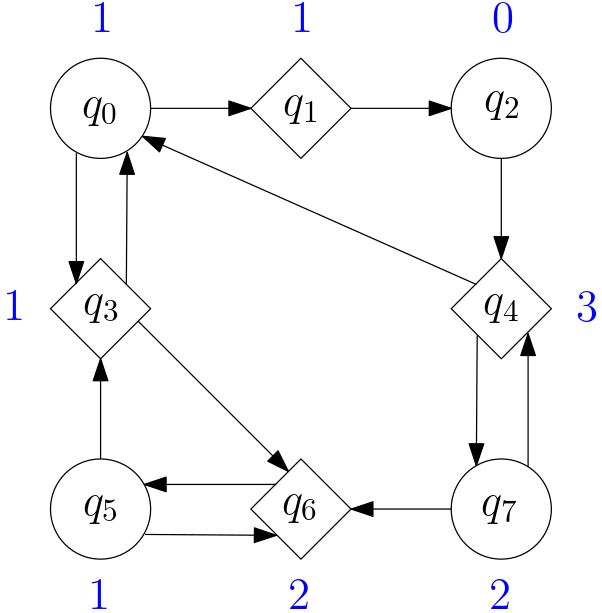
\includegraphics[width=0.4\textwidth]{figures/parity_game}
	\caption{An example of an arena. Circles  belong to player $0$, whereas diamonds belong to player $1$. Arrows represent transitions from a configuration to the next. The priority assigned by the priority mapping to each configuration is a number in $\{0,1,2,3\}$, next to the configuration it is assigned to. Note that we do not have a dead end in our example.}
	\label{example_parity_game}
	\end{figure}
\end{center}

\begin{example}
Let us consider the arena presented in  Figure~\ref{example_parity_game}. 
Configurations are partitioned into two sets: the circles, belonging to player $0$, and the diamonds,
belonging to player $1$. 
The priorities are $\{ 0,1,2,3\}$.
% The transitions and priority mappings may be derived from the picture.
% Note that we don't have a dead end in our example. 
Consider the game on the arena, where the winning condition is a parity condition.
Plays $\pi_1 = q_0 q_1 q_2 (q_4 q_7)^\omega$ and 
$\pi_2 = (q_0 q_1 q_2 q_4)^\omega$ are both winning for player $0$. Indeed, in $\pi_1$, 
the minimal priority encountered infinitely often is %that of $q_7$, that is, 
				$2$, 
whereas in $\pi_2$, it is %that of $q_2$, that is, 
			$0$. 
In both cases, it is an even number. On the other hand,
the plays $\pi_3 = (q_5 q_3 q_6)^\omega$ and $\pi_4=(q_5 q_6)^\omega$ are both winning for player $1$: the minimal priority encountered is odd, since it is $1$ for both.

One can take matters further: on this arena, player $0$ has a winning strategy for the parity game from $q_0$, $q_1$, $q_2$, $q_4$ and $q_7$, but not from $q_5$, $q_3$ nor $q_6$, where player $1$ has a winning strategy. 
\end{example}



% \mh{Say something abut positional determinacy}
One important property of parity games is that of {\em memoryless determinacy}: for a parity game
$\mathcal{G}= ((S_0,S_1,\rightarrow),\win_\Omega) $ and an initial configuration $s \in S_0 \cup S_1$, one of the players has a memoryless winning strategy from $s$ \cite{zielonka1998infinite}.

%\mh{
Of note is that several model checking problems %for pushdown automata 
can be expressed as decision problems for games: the most famous example is that the modal $\mu$-calculus model checking problem is polynomially equivalent to solving the parity game problem. 
%}



% \subsection{Complexity}
\section{Complexity}

We assume the reader is familiar with 
Turing machines% and standard complexity classes such as $\LOGSPACE$, $\PSPACE$ and $\EXPSPACE$. We refer to \cite{Papa94,AroBar09} for further details on complexity
.
%\iffalse
A proper definition of space bounded deterministic Turing machines is provided in 
Section~\ref{DTMs}, 
where a more thorough analysis of their behavior is required.
%\fi



We now provide an overview of time and space complexity classes. 
% The {\em running time} of a Turing machine is a function $f : \N \rightarrow \N$ such that for any input word $w$ of size $n$, the length of any computation on $w$ is at most $f(n)$. 
We say a Turing machine is
{\em $f(n)$-time bounded} if %its running time is $f$.
for any input word $w$ of size $n$, the length of any computation on $w$ is at most $f(n)$. 
We say a Turing machine is
{\em $f(n)$-space bounded} if $f(n)$ is the size of its working tape 
for any computation of the Turing machine on an input of length $n$.


 
% In the following, we assume the reader is familiar with other complexity classes such as
By $\P$, and $\EXP$ we denote the classes of all problems that can be decided by a deterministic Turing machine who is polynomially or exponentially time bounded, respectively and
by
 $\NP$, and $\NEXP$ we denote the classes of all problems that can be decided by a non-deterministic Turing machine that is polynomially or exponentially time bounded, respectively. 

By ${\sf L}$, $\PSPACE$, and $\EXPSPACE$ we denote the classes of all problems that can be decided
by a deterministic Turing machine that is logarithmically, polynomially, exponentially space bounded, respectively. We do not explicitly define 
$\NPSPACE$ and $\NEXPSPACE$
since by Savitch’s theorem \cite{Sav70} they are equivalent to 
$\PSPACE$ and $\EXPSPACE$ respectively.
We do however define ${\sf NL}$ as the 
class of all problems that can be decided
by a nondeterministic Turing machine that is logarithmically space bounded.


% We abuse notations and say a language $L$ is in a complexity class if the problem of whether or not a word $w$ belongs to $L$ is itself in the complexity class.
%
%

% \def\powertower#1#2{#1\ifnum#2>1 ^{\powertower{#1}{\numexpr#2-1\relax}}\fi}
% $\powertower{2}{5}$


We define the tower function $T : \N \times \R \to \R$ by $T(0,r) =r$ and
$T(h+1,r)= 2^{T(h,r)}$ for all $h \in \N, r \in \R$. Thus $T(h,r)$ is a tower of $2$s of height $h$ with an $r$ sitting on top, i.e.

\iffalse
$$\text{height } h \begin{cases}&  2^{2^{2^{2^{2^{2^{2^
	 {{\hspace{0.13cm}}^{\cdot^{{\hspace{0.13cm}}^{\cdot^{
	 {\hspace{0.13cm}}^{\cdot^{{\hspace{0.13cm}}^{2^{2^{2^{2^r}}}}}}}}}}}}}}}}} 
	 = T(h,r)
	\end{cases} $$
\fi	
	
$$	 \left.
    \begin{array}{ll}
T(h,r) = 2^{2^{2^{2^
	 {{\hspace{0.13cm}}^{\cdot^{{\hspace{0.13cm}}^{\cdot^{
	 {\hspace{0.13cm}}^{\cdot^{{\hspace{0.13cm}}^{2^r}}}}}}}}}}} 
    \end{array}
\right \} \text{height } h $$

% https://math-linux.com/latex-26/faq/latex-faq/article/horizontal-and-vertical-curly-braces-left-right-underbrace-and-overbrace

Observe that for all $n,h \in \N$ with $n\geq 1$, we have
$T(h, log^{(h)}(n)) = n$.
%
% 
Here a problem is in {\sf ELEMENTARY} if there exists $h \in \N$ such that
it can be solved in time $O ( T(h, 0) )$. By $h$-$\EXP$ we denote the class of all problems that can be decided by a deterministic Turing machine who is $T(h,f(n))$-time bounded for some polynomial function $f$.
% k-EXP is the union of DTIME(2^{n^i}_k ), for i ≥ 1.
The complexity class %$h$-$\NEXP$, 
$h$-$\EXPSPACE$ 
%and $h$-$\NEXPSPACE$ 
is defined analogously.


Finally, by $\PSPACE^\NEXP$ we denote the class of all problems that can be decided by a deterministic Turing machine that is polynomially space bounded, and that has access to results from an oracle  in $\NEXP$.

A true/false problem is {\em decidable} if there exists a 
time bounded Turing Machine 
% \textcolor{black}{for which all computations end in a finite number of steps and answer yes or no to the question asked by the problem.} 
that answers the question asked by the problem.
If there exists no such Turing Machine, the problem is {\em undecidable}. \\

\par\noindent\ignorespacesafterend
For a complexity class $C \in \{ \NP, \PSPACE, \NEXP, \PSPACE^\NEXP, \EXPSPACE, h-\EXP, h-\EXPSPACE\}$, we say a problem $P$ is {\em $C$-hard} when every problem in $C$
can be reduced in polynomial time to $P$. For a complexity class $C \in \{{\sf NL}, \P\}$
we 
say a problem $P$ is {\em $C$-hard} when every problem in $C$
can be reduced to $P$ using logarithmic space only.
When a problem $P$ is both $C$-hard and in $C$,
we call it {\em $C$-complete}. 



 %
For more information on Turing machines in the broader definition, we refer the reader to  \cite{Papa94,AroBar09}, which provide further details on complexity theory as well. 
% Space bounded deterministic Turing machine will be introduced in more details in Section~\ref{DTMs} where a more thorough analysis of their behavior is required.


% \subsection{Automata}
\section{Automata}


\begin{samepage}
A {\em finite automaton}  is a tuple
$\A=(Q,\Sigma,R,q_{init},F)$, where
\begin{itemize}
	\item $Q$ is a finite {\em set of  states}, 
	\item $\Sigma$ is a {\em finite input alphabet},
	\item $R\subseteq Q\times \Sigma \times Q$
	is a %finite {\em set of  rules},
		{\em transition relation},
	\item $q_{init}\in Q$ is the {\em initial  state}, and 
	\item $F\subseteq Q$ is a {\em set of final  states}. \newline
\end{itemize}
\end{samepage}

\noindent
A finite automaton $\A=(Q,\Sigma,R,q_{init},F)$
 induces the finite labeled transition system $(Q, \Sigma, R)$.

The {\em size} of $\A$ is defined as $|\A| \ = \ |Q|+|\Sigma|+|R|$.

A {\em run} from $q_0$ to $q_n$ in $\A$ is a 
path in the labeled transition system $(Q, \Sigma, R)$ induced by $\A$,
and will be noted
$q_0 \xrightarrow{a_0} q_1 \xrightarrow{a_1} \cdots \xrightarrow{a_{n-1}} q_n$,
for $a_0, \ldots, a_{n-1} \in \Sigma$.
We sometimes use the abbreviation $q \rightarrow^* q'$
to denote a run of arbitrary length from $q$ to $q'$.
We say $\pi$ is {\em accepting} if
 $q_0 = q_{init}$
 and $q_n \in F$.
% We say {\em reachability holds} for $\A$ if there is an accepting path in $\A$.

We say a word $w \in \Sigma^*$ is accepted by $\A$ if 
$q_{init} \xrightarrow{w} q$ in $(Q, \Sigma, R)$
for some $q \in F$. % \mh{defined in the section about Transition systems}
%
The {\em language} of $\A$ is $L(\A)$ the
set of elements accepted by $\A$.
We say a language $L$ is {\em regular} if there exists a finite automaton $\A$
such that $L= L(\A)$.

\begin{center}
	\begin{figure}
			\hspace{3.81cm}
\includegraphics[width=0.4\textwidth]{figures/example_automata}
	\caption{A finite automaton that accepts $\{a,b\}^*ab\{a,b\}^* $. The automaton consists of three states, the input alphabet is $\{a,b\}$. The transitions are represented by arrows labeled with the corresponding input symbol. The initial state is $q_0$ and the set of final state is composed of the singular  state $q_f$.}
	\label{example_automata}
	\end{figure}
\end{center}

\begin{example}
	See Figure~\ref{example_automata} for an example of an automaton that accepts the language $\{a,b\}^*ab\{a,b\}^* $.
\end{example}

We are interested in the following decision problem.

\problemx{Automata reachability}
{A finite automaton $\A$.}
{Does 
%reachability hold for
there exists an accepting run in
 $\A$?\newline}


We refer the reader to \cite{Har78} for more details on
 %(deterministic) 
 finite automata and regular languages. \newpage











